\documentclass[a4paper]{report}
\author{Jure Kos}
\title{Vaja 10, Težni pospešek}
\date{25.11.2021}
\usepackage{graphicx}
\graphicspath{ {./images/} }

\begin{document}

\maketitle

\chapter*{Uvod}
Na telo z maso m deluje teža, ki je sorazmerna z maso:

\[F = mg\]\\

Če ni drugih zunanjih sil, telo po Newtonovem zakonu enakomerno pospešeno pada s pospeškom g. Iz lastnosti enakomerno pospešenega gibanja vemo, da je pot po času t podana z:

\[s=\frac{gt^2}{2}+v_0t\]

če se je telo ob času $t = 0$ premikalo s hitrostjo v0.

\section{Naloga}
1. Preveriti, da je prosti pad enakomerno pospešen.\\
2. Izračunati težni pospešek.\\

\section{Potrebščine}
1. Elektronska ura,\\
2. dve optični stikali,\\
3. elektromagnet,\\
4. stojalo,\\
5. jeklena kroglica,\\
6. dva izvira enosmerne napetosti.

\chapter*{Potek}
Kroglico magnetno obesimo pod konico elektromagnetnega držala. Ko se kroglica umiri preklopimo stikalo. Trenutek za tem se kroglica odlepi od konice jedra in pade mimo dveh optičnih stikal na tla. Rezultat na uri prepišemo. Opravimo nekaj testnih meritev, da ugotovimo, do katerega decimalnega mesta je čase smiselno prepisovati. Pomembno je, da določimo dolžino poti kroglice čim bolj natančno. Opravimo vsaj 50 meritev. Interval med najkrajšim in najdaljšim odčitkom časa razdelimo na 10 enakih delov. Število poskusov, ki padejo v en interval, deljeno
s celotnim številom poskusov limitira pri naraščajočem številu meritev proti verjetnosti, da meritev pade v ta časovni interval. Pričakujemo normalno (Gaussovo)
verjetnostno porazdelitev, ki se opiše z naslednjo verjetnostno gostoto (verjetnost
na enoto intervala):

\[\omega(x)=\frac{1}{\sqrt{2\pi}\sigma}e^{-\frac{(x-\overline{x})^2}{2\sigma^2}}\]

Pri tem je $\sigma$ efektivni odmik in $\overline{x}$ povprečna vrednost. Narišemo na isto sliko še ustrezno krivuljo za normalno porazdelitev. Verjetnost, da pade meritev v ozek časovni interval med $t'-\frac{dt}{2}$ in $t'+\frac{dt}{2}$ je enaka

\[P\left(t'-\frac{dt}{2}<t<t'+\frac{dt}{2}\right) =\omega(t')dt\]
\pagebreak
\chapter*{Meritve}
Izmerjene čase zapišemo v tabelo.\\

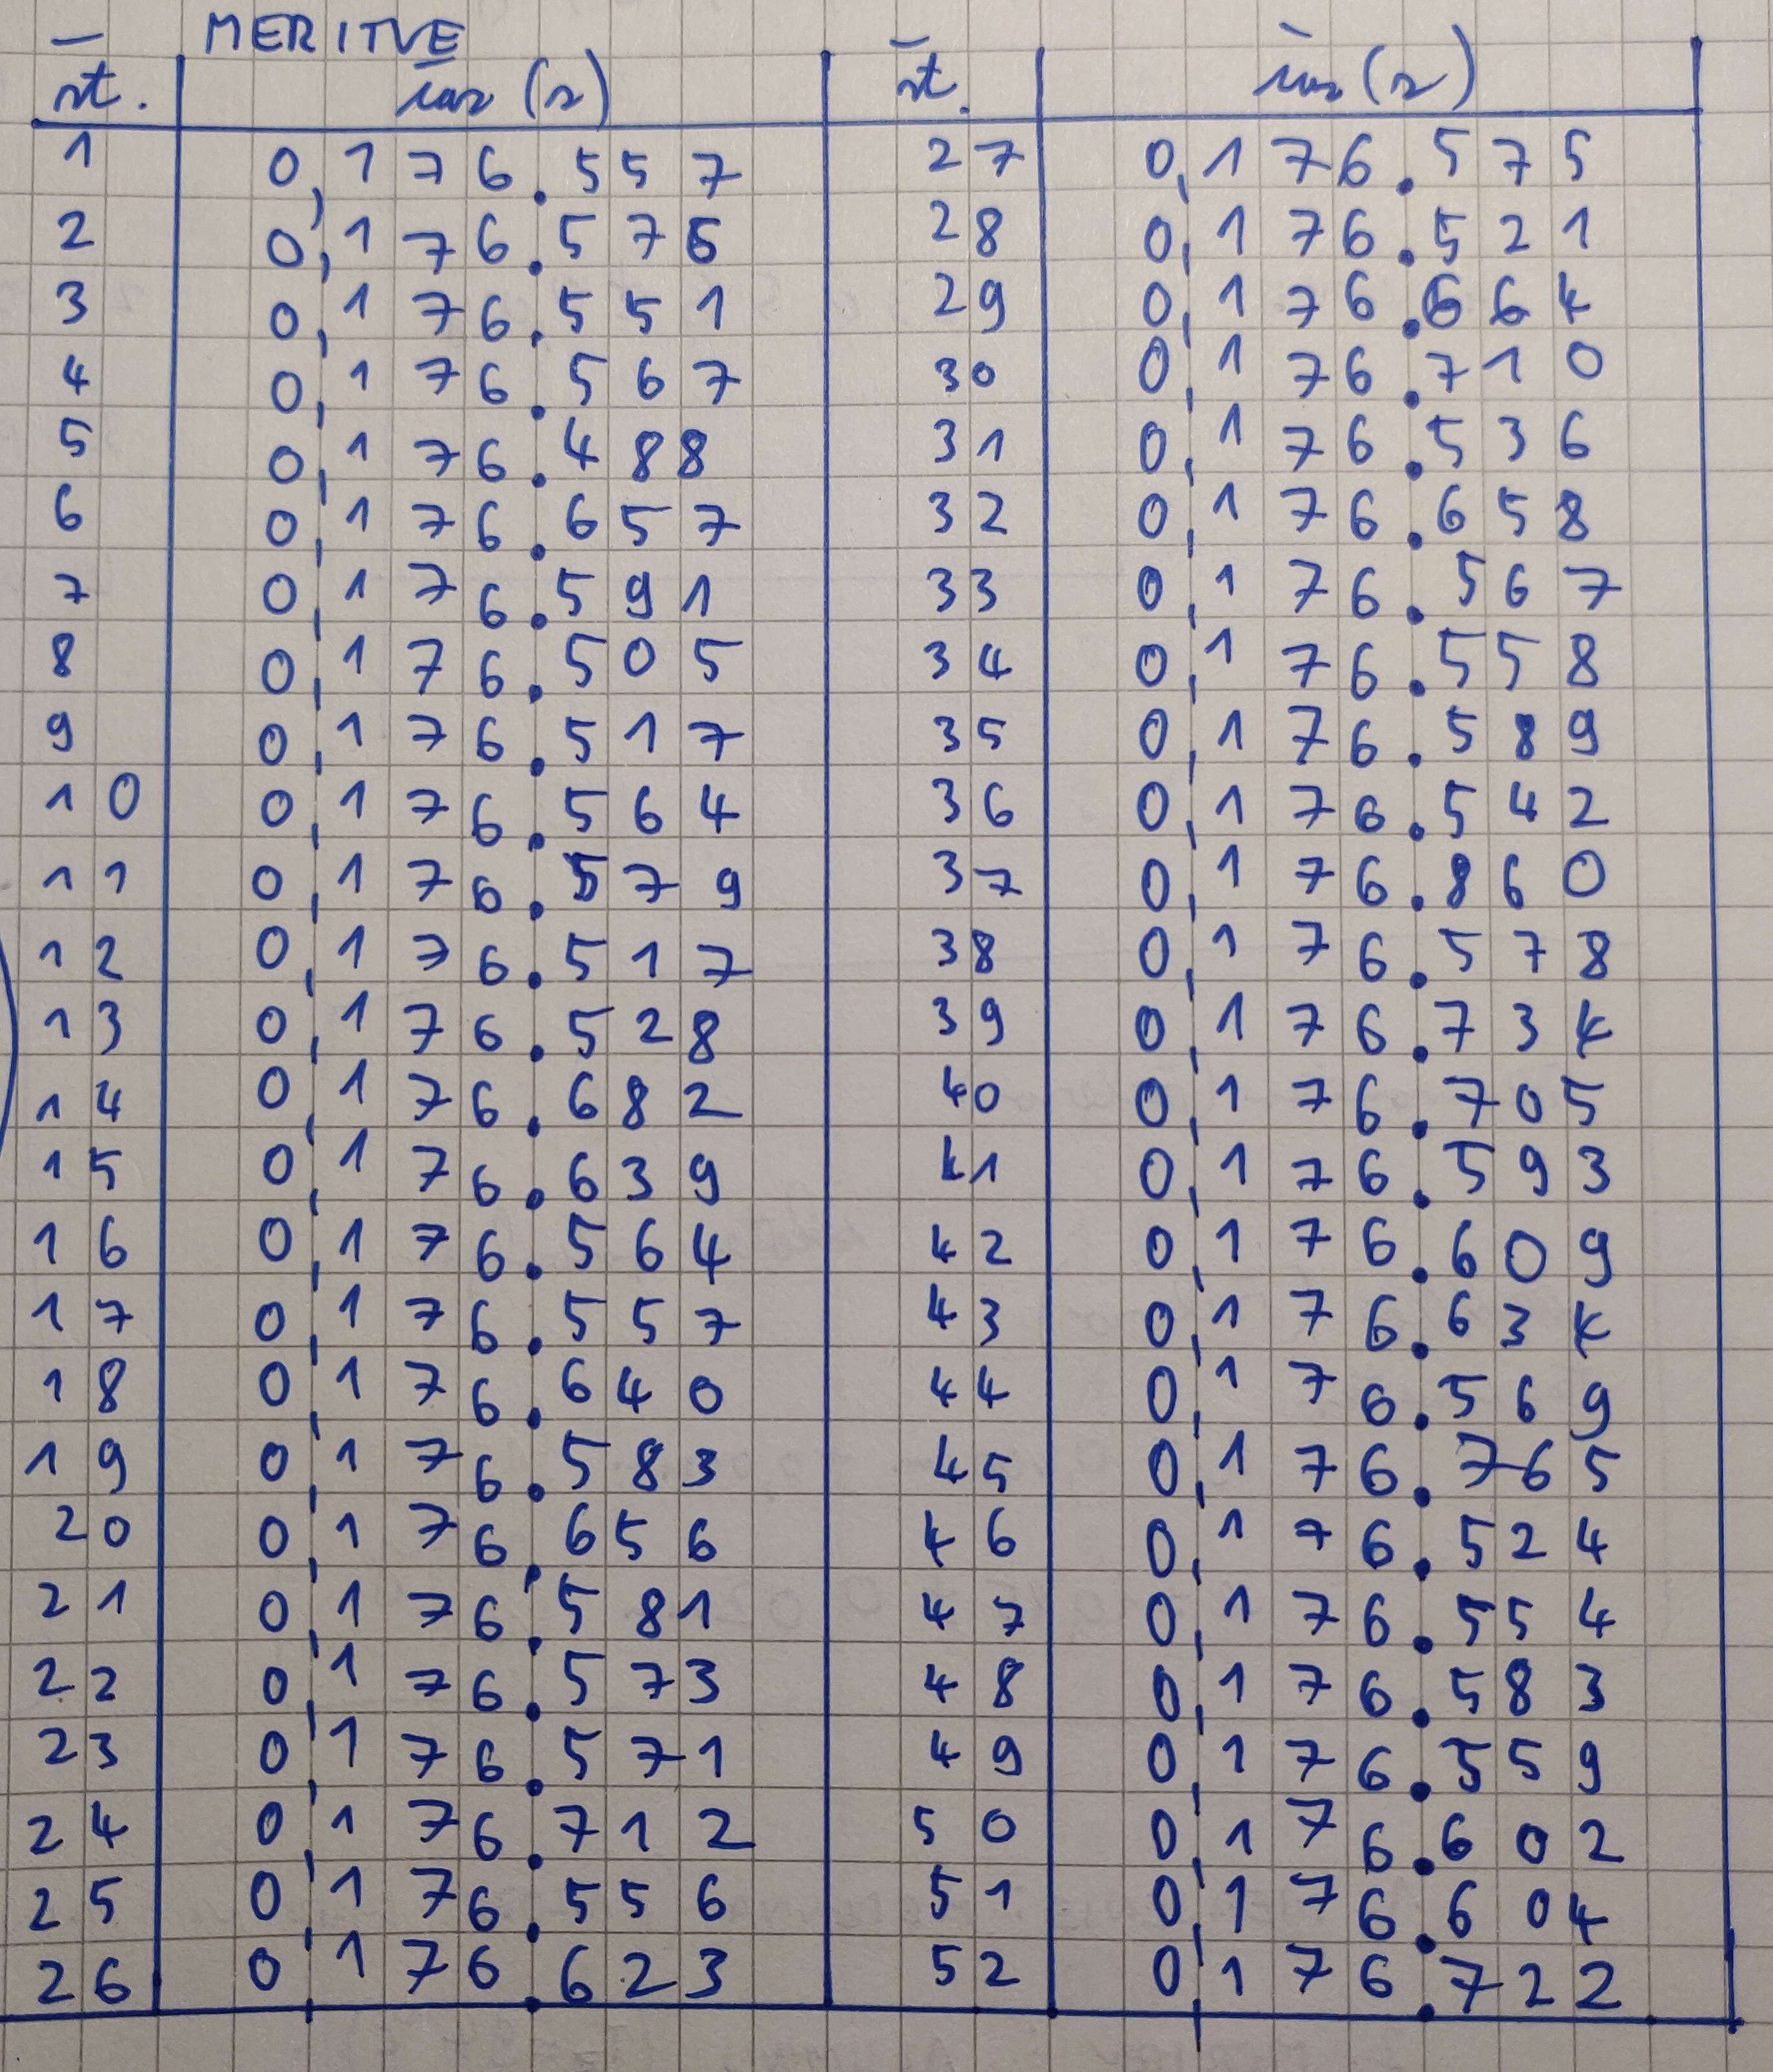
\includegraphics[width=\textwidth]{Tabela meritev}
Poleg tega smo višino 1 med kroglico in prvimi vrati izmerili kot $3.65cm\pm0.11cm$\\
Višino 2 med optičnimi vrati pa kot $29,86cm\pm0,11cm$
\pagebreak

Meritve razdelimo na 10 intervalov glede na zadnje 3 decimalke.\\
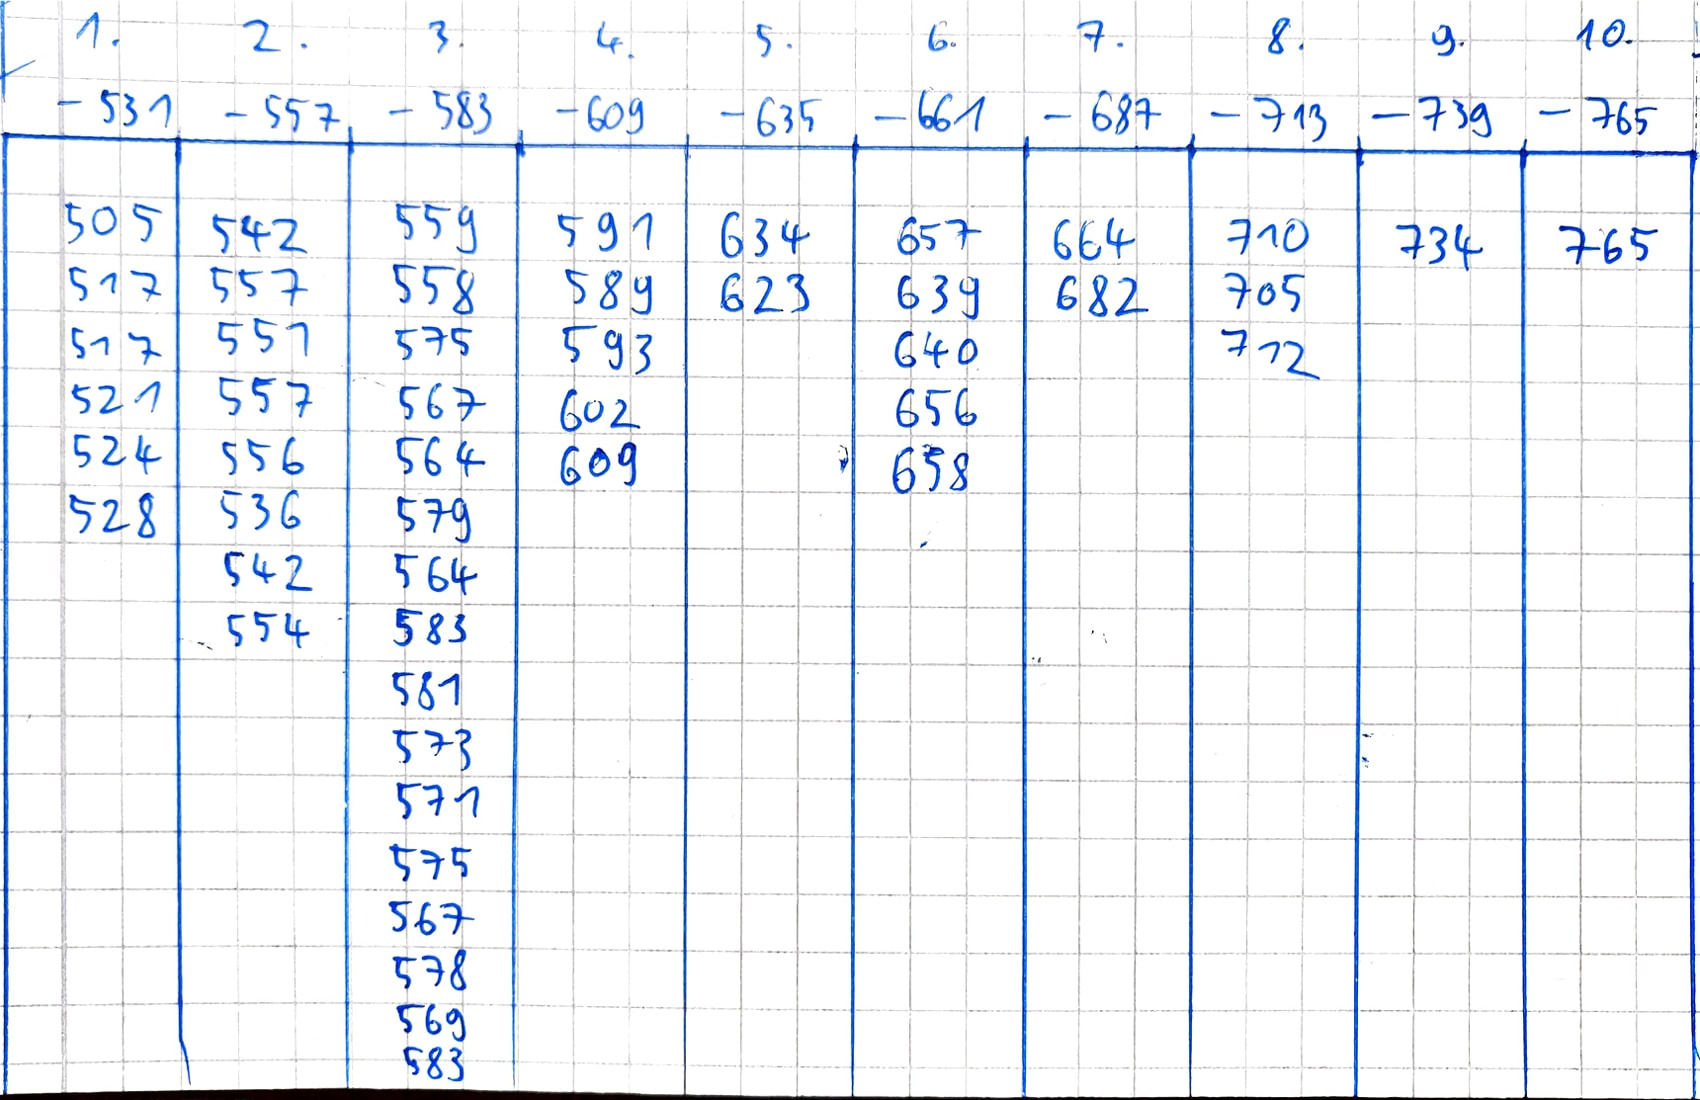
\includegraphics[width=\textwidth]{Tabela intervalov}

\chapter*{Računi}
Najprej izračunamo povprečen čas padanja med merilnikoma.

\[\overline{t}=\frac{\sum_{n=1}^{50}t_n}{50}=0,176.572s\]

Po enačbi za prosti pad je:
 \[h_2=v_0t+\frac{gt^2}{2}=\sqrt{2gh_1}t+\frac{gt^2}{2}\]
 
 \[h_2-\frac{gt^2}{2}=\sqrt{2gh_1}t\]
 
 \[\frac{g^2t^4}{4}-gt^2(h_2+2h_1)+h_2^2\]
 Če to obravnavamo kot kvadratno enačbo za g dobimo enačbo
 
 \[g=\frac{2}{t^2}\left(h_2+2h_1-2\sqrt{h_1h_2+h_1^2}\right)\]
 Ko v dobljeno enačbo vstavimo podatke, dobimo za rezultat 
 \[g=9,65m/s^2\pm 0,53m/s^2\]
 
\chapter*{Grafi}
Ko v graf vstavimo dobljene meritve po intervalih Dobimo stolpično porazdelitev ki ustreza izračunani normalni porazdelitvi okoli povprečne vrednosti izmerjenega časa.\\
 
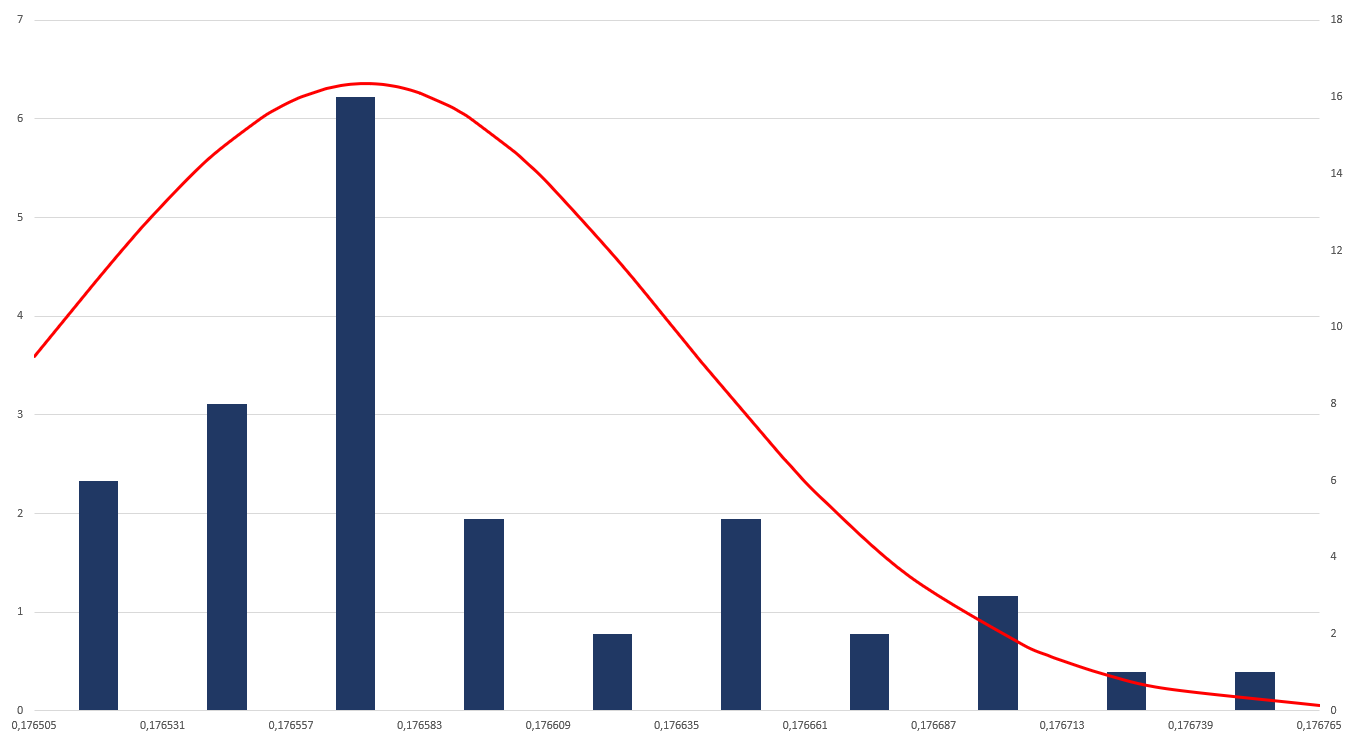
\includegraphics[width=\textwidth]{Normalna porazdelitev}
 
\chapter*{Odgovori na vprašanja}
 \section*{Kako je negotovost dobljenega rezultata odvisna od razdalje med optičnimi vrati in višine, s katere spustimo kroglico?}

Negotovost rezultatov je odvisna od napake narejene pri merjenju časov in razdalj. Ker je napaka pri času znatno manjša od napake pri razdalji na negotovost bolj vpliva napaka pri merjenju razdalj. Relativna napaka dolžine se obratno sorazmerno povečuje z razdaljo med optičnimi vrati.
\\

Celotna izračunana vrednost pa odstopa tudi zaradi negotovosti hitrosti pri zgornjih vratcih. Večja kot je razdalja med mirovno lego in zgornjimi vratci večja je negotovost rezultata.
\\
\section*{Kako nastaviti razdalje, da bo negotovost končnega rezultata čim manjša?}

Razdaljo med vratci bi povečali da bi se relativna napaka zmanjšala, razdaljo med začetno lego žogice in prvimi vratci pa bi zmanjšali, da bi žogica prečkala prva vratca s čim manjšo hitrostjo.


\end{document}
